% $Header$

\documentclass{beamer}

% Copyright (c)  2021  HiKlas Ltd.
% Permission is granted to copy, distribute and/or modify this document
% under the terms of the GNU Free Documentation License, Version 1.3
% or any later version published by the Free Software Foundation;
% with no Invariant Sections, no Front-Cover Texts, and no Back-Cover Texts.
% A copy of the license is included in the section entitled "GNU
% Free Documentation License".
%
% Based on the Beamer generic-ornate-15min-45min.en.tex template by
% Till Tantau <tantau@users.sourceforge.net>



\mode<presentation>
{
  \usetheme{CambridgeUS}
}

\usepackage[english]{babel}
\usepackage[latin1]{inputenc}
\usepackage[T1]{fontenc}
% Or whatever. Note that the encoding and the font should match. If T1
% does not look nice, try deleting the line with the fontenc.

% These packages are used for drawing circuits
\usepackage{tikz}
\usepackage[siunitx,european,americanresistors]{circuitikz}

% Packages for mathematical notation
\usepackage{amsmath}

% Information about the presentation 
\title{Introduction to Machine Code}
\subtitle{003 6502 CPU}
\author{Fiona Bianchi}
\institute{HiKlas Ltd}
\date{August 2021}
\subject{Talks}
\pgfdeclareimage[height=0.5cm]{company-logo}{../assets/HiklasLogo.eps}
\logo{\pgfuseimage{company-logo}}

% Table of contents for each Subsection
\AtBeginSubsection[]
{
  \begin{frame}<beamer>{Outline}
    \tableofcontents[currentsection,currentsubsection]
  \end{frame}
}

% TODO: Nope, I don't think I want this put leaving it in just in case
% TODO: to remove when absolutely sure
% If you wish to uncover everything in a step-wise fashion, uncomment
% the following command: 
%\beamerdefaultoverlayspecification{<+->}

% Show the notes
\ifdefined\isnotes
  \setbeameroption{show only notes}
\fi

% Show notes and slides
\ifdefined\ishandout
\setbeameroption{show notes}
\fi

\begin{document}

\begin{frame}
  \titlepage
\end{frame}

\begin{frame}{Outline}
  \tableofcontents
  % TODO: What is "pausesections" for?
  % You might wish to add the option [pausesections]
\end{frame}


\section{6502 Central Processor Unit}

\subsection[History]{History}

\begin{frame}{A frame}
  \begin{itemize}
  \item
    One item
  \item
    Two item
  \end{itemize}
\end{frame}


\subsection[Appearance]{What does it look like?}

\begin{frame}{Chip Pinout}
  \begin{columns}
    \column{0.50\textwidth}
    \begin{itemize}
    \item
      One item
    \item
      Two item
    \end{itemize}

    \column{0.50\textwidth}
    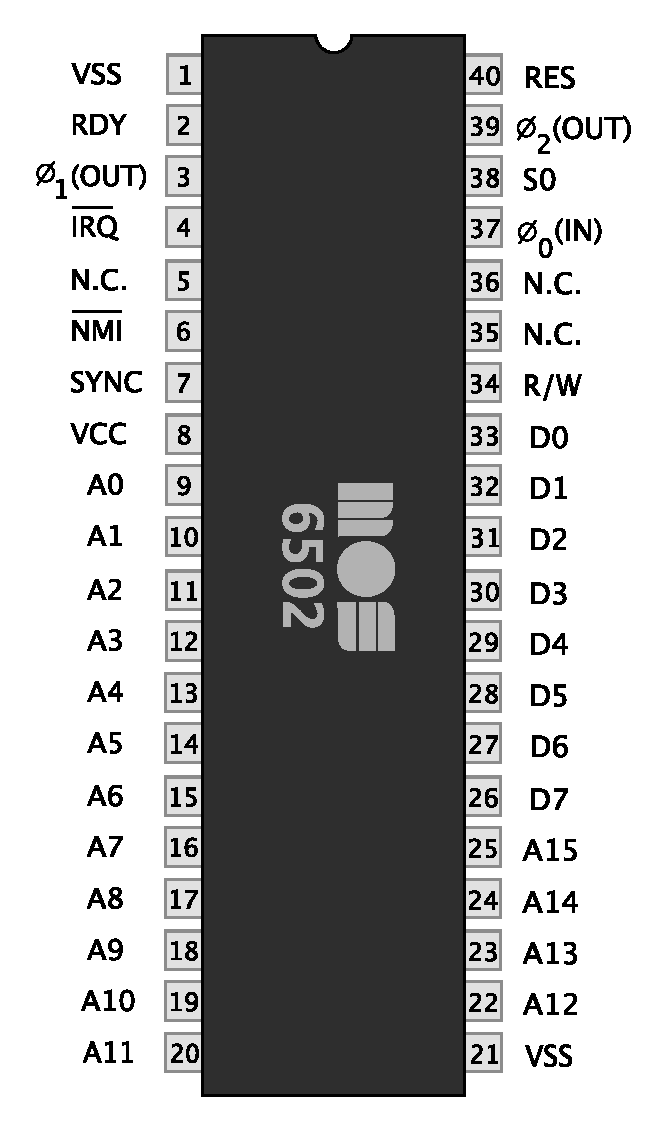
\includegraphics[scale=0.25]{../assets/MOS6502.eps}
    
  \end{columns}
\end{frame}

\begin{frame}{Chip Die}
  \begin{columns}
    \column{0.25\textwidth}
    \begin{itemize}
    \item
      One item
    \item
      Two item
    \end{itemize}

    \column{0.75\textwidth}
    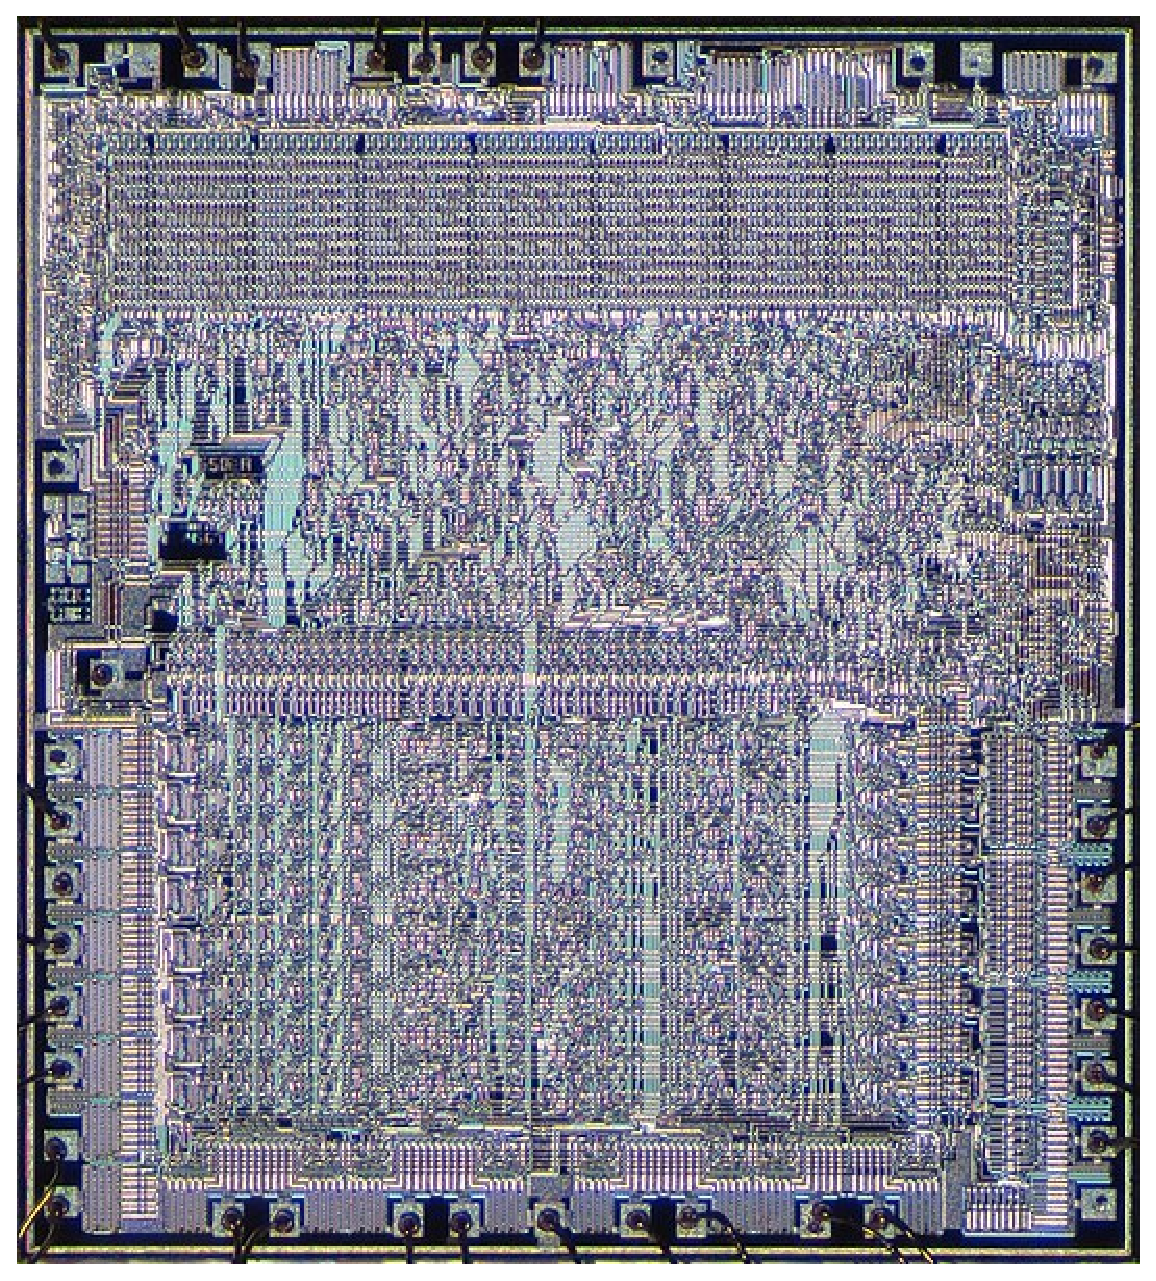
\includegraphics[scale=0.25]{../assets/MOS_6502_die.eps}
    
  \end{columns}
\end{frame}


\subsection[Internals]{What's inside?}

\begin{frame}{Processor Die}
  \begin{itemize}
  \item
    One item
  \item
    Two item
  \end{itemize}
\end{frame}


\section{Programming}

\subsection[Instructions]{Instructions}

\begin{frame}{A frame}
  \begin{itemize}
  \item
    One item
  \item
    Two item
  \end{itemize}
\end{frame}


\subsection[Interupts]{Getting interrupted}

\begin{frame}{A frame}
  \begin{itemize}
  \item
    One item
  \item
    Two item
  \end{itemize}
\end{frame}


\section{Emulator}

\subsection[GettingStarted]{Getting Started}

\begin{frame}{A frame}
  \begin{itemize}
  \item
    One item
  \item
    Two item
  \end{itemize}
\end{frame}

\subsection[Examples]{Example Code}

\begin{frame}{A frame}
  \begin{itemize}
  \item
    One item
  \item
    Two item
  \end{itemize}
\end{frame}




\section{Summary}

\begin{frame}{Summary}

  % Keep the summary *very short*.
  \begin{itemize}
  \item
    Item one
  \item
    Item two
  \end{itemize}
  
  % The following outlook is optional.
  \vskip0pt plus.5fill
  \begin{itemize}
  \item
    Outlook
    \begin{itemize}
    \item
      Something you haven't solved.
    \item
      Something else you haven't solved.
    \end{itemize}
  \end{itemize}
\end{frame}

\section{Bibliogrphy}

\begin{frame}{Bibliography 1}
  \frametitle{References}
  \begin{thebibliography}{MOS 6502 Die}
  \bibitem[MOS 6502 Die]{MOS6502Die}
    Die image: {\url{https://commons.wikimedia.org/wiki/File:MOS_6502_die.jpg}}
  \bibitem[MOS 6502 Chip]{MOS6502Chip}
    Chip image: {\url{https://commons.wikimedia.org/wiki/File:MOS6502.svg}}
  \bibitem[6502 Wikipedia Page]{6502Wikipedia}
    Wikipedia: {\url{https://en.wikipedia.org/wiki/MOS_Technology_6502}}
  \end{thebibliography}
\end{frame}


\end{document}


